
\documentclass[14pt, oneside]{article}   	% use "amsart" instead of "article" for AMSLaTeX format
\usepackage{geometry}                		% See geometry.pdf to learn the layout options. There are lots.
\geometry{letterpaper}                   		% ... or a4paper or a5paper or ... 
\usepackage{makeidx}

\usepackage{amsmath,amsfonts,amsthm} % Math packages
\usepackage[pdftex]{graphicx}	
\usepackage{url}
		
\usepackage{amssymb}
\usepackage{subfigure}
\usepackage{tabularx}
%\usepackage{asmthm}
\usepackage{program}
\newtheorem{Lem}{Lemma}
\newtheorem{Them}{Theorem}
\newtheorem{Conj}{Conjecture}

\newcommand{\horrule}[1]{\rule{\linewidth}{#1}} 

\title{ \horrule{0.5pt} \\[0.4cm] \huge Cancelable Biometrics: Fingerprint Shell combined with Quantization and Bit String generation \\ \horrule{1.5pt} \\[0.1cm]}
\author{Chinthamreddy premsai}
\date{\today}

%%% BEGIN DOCUMENT
\begin{document}
\maketitle
\newpage
\section*{\textbf{Certificate}}
\newpage
\setcounter{tocdepth}{3}
\tableofcontents
\newpage

\section{Introduction}
Biometrics has become one of the greatest tools ever known to mankind to defend his own identity.  Among biometrics fingerprint plays an important role in day today use. In day today life we use fingerprint to record attendance of employees, students in large organisations. Now a days banks are starting to use fingerprint for some of the transactions. Also fingerprints play an important to relate a criminal to a crime scene.
\paragraph{}
All biometric systems consists of two main phases, Enrollment phase and Matching phase. In enrollment phase the user's identity is enrolled with the system. All the enrolled identities are stored in a database in some format. In the matching phase user's input is again collected and is matched with the already enrolled identities in the system in the enrolment phase. 
\subsection{Enrollment}
Collecting biometric features from a user and storing it in the system to use for later is the main purpose of enrollment phase. The collected biometric sample can be stored either in the raw form or with transformations made to it. The biometric features are collected using sensors and the collected samples are preprocessed before storing using different algorithms based on what kind of biometric trait we are using. These stored templates are matched with the query templates to test for genunity and imposterness. 
\subsection{Matching}
\textit{Indentification} and \textit{Verification} are the two kinds of identity management functionalities provided by any biometric system. 
\paragraph{}
Verification is the task of verifying the identity of the user based on the user input and his claimed identity. This identity can be his name, username, Personal Identification Number(PIN) or a token. Verification is a one to one match, where the user's input is compared only with the claimed identity already stored in the system.  The user is said to be \textit{Genuine} if a particular percentage of biometric features from user's input matches with the already enrolled features in the system or else the user will be declared as an \textit{Imposter}. 
\paragraph{}
Identification can be classified into two categories, one is positive identification and the other is negative identification. In positive identification the system checks whether the user's input is matching with any of the identities that are already known to the system. If the user's input of biometric features matches with any of the identities then the user is considered as a genuine user or else will be considered as an imposter.  The negative identification is also called screening. In this identification, the user's input is matched with all the system known identities. If any of the system known identities matches with the user's input then the user is  said to be an imposter unlike in the positive identification. This type of identification is used to regulate criminals in the watch list to leave the country by installing systems in the airports. \cite{1}
\subsection{Template Protection}
After the biometric features are collected from the user, these are needed to be stored in the database. The way in which these templates are stored is one of the major issues we are facing in the biometric systems. We are talking mainly about fingerprints among all the biometric features. After collecting fingerprints from the sensor, the templates are needed to be stored. If the fingerprint images are directly stored in the database and if the database is compromised the user's fingerprint will be known which will be potentially dangerous. If a database storing passwords is compromised, by changing the password we can revoke the privilege to any particular system. But if the database with fingerprint templates is compromised and if the attacker is able to figure out how the fingerprint looks like then the user's identity can be considered to be stole. The user cannot change his fingerprint, so he cannot revoke the permissions in any system. So we need a fingerprint storing format from which the chances of getting the original fingerprint image are highly impossible. Any template protection scheme should have all the four properties that are discussed below:\cite{2}

\begin{description}
  \item[Revocability] \hfill \\
  Even if the template are compromised, the user should be able to reuse his same fingerprint to generate a new template.
  \item[Diversity] \hfill \\
  If two systems are using the same template generation method, the template in one system should not correspond to the respective user template in another system.
  \item[Accuracy] \hfill \\
  The templates should be generated in such a way that matching a user with his generated template should be accurate.
  \item[Irreversible]\hfill \\
  The new template should not reveal the information to reverse engineer the fingerprint corresponding to it. It should be irreversible.
\end{description}

Jain et al. (2008) have classified the template protection schemes into three main categories: \textit{Feature Transformation, Biometric crypto systems and Hybrid}.  Each scheme has it's own advantages and limitations according to the survey of Rathgeb Christian and Uhl Andreas ,2011. \cite{2}. All these schemes should meet all the four requirements of an ideal protection scheme. we are concerned with the feature transformation approach in this text.  The basic idea of feature transformation approach is to transform the features of the original biometric sample \textbf{$T$} using a transformation function \textbf{$F$} and a key \textbf{$K$}; the transformed template \textbf{$F(T,K)$} is then stored in the database. The function \textbf{$F$} is applied to the query the template and the transformed query template \textbf{$F(Q,K)$} is compared directly with the transformed template already stored in the database. 
\paragraph{}
In this paper we propose a new non-invertible feature transformation technique for the template protection. Also this template protection scheme is less sensitive to translation and rotation, an alignment free fingerprint template protection technique. 
\paragraph{}
In section $2$, we review the template protection schemes. The proposed approach is presented in section 3. Our experimental results and comparisons are presented in section $4$. Our conclusions and future work are in section $5$.
\section{Related Work}
Fingerprint systems that are based on minutiae of the fingerprint, mainly consists of three steps. Initially the fingerprint image collected from the sensor is pre-processed ( i,e., Segmentation, binarization, thinning, etc.). Secondly the feature extraction phase where the minutiae of the fingerprint like ridge endings, bifurcations, Cores and Deltas. Finally fingerprint matching should be done with or without alignment and the matching scores are generated.  If the minute information (i.e., coordinates and orientations are stored in the database, according to some research works the original fingerprint impression can be reconstructed using that information ( Ross et al., 2005; Cappelli et  al., 2007)\cite{3}. Thus the design of new protection techniques has become increasingly important.
\paragraph{}
In practice fingerprints among the same user have more variations due to translation and rotation of fingerprint impressions during collection. Many of the methods proposed are alignment free techniques because of the difficulty in aligning the fingerprint based on core or delta in the fingerprint. Also many of the fingerprint do not contain cores and deltas which may lead to higher rejection rate if the alignment is based on cores and deltas. Therefore, fingerprint recognition is very sensitive to orientation and translation of impressions which makes fingerprint template protection more complicated. \cite{4}
\paragraph{}
Ratha et al. introduced registration-based cancelable fingerprint template schemes using three non-invertible transformations\cite{5} . Feng et al. \cite{6}  and Shin et al. \cite{7} argued that the cancelable template schemes proposed by Ratha are vulnerable, especially the surface-folding functional transformation. Feng launched a solving- equation attack  while Shin launched a brute force attack by trying all possible points in the original fingerprint image.\cite{8}
\paragraph{}
Some proposed a new secure representation from the minutiae representation. Ferrara, Maltoni and Cappelli in 2012 proposed a protected version of Minutiae Cylinder Code (MCC) which is a new fingerprint template representation\cite{9}. A cylinder for each minutiae is used to encode spatial and directional information between the minutiae and it's neighbourhood and create the fingerprint template.
Ferrara et al.\cite{10} then proposed a recovery algorithm to derive the original minutiae from the MCC template and further proposed  a non-invertible scheme, namely protected minutia cylinder code (P-MCC) by using the binary principal component analysis. Although the non-invertibility of P-MCC template has been experimentally justified, P-MCC is still unable to protect the genuine minutiae points. It is shown in \cite{10} that a portion of genuine minutiae (approximately $25.4\%$) can still be precisely recovered.
\paragraph{}
Lee et al. \cite{11} proposed a cancellable fingerprint template using fingerprint minutiae. A 3-dimensional array is first defined and the number of cells contained in the 3D array are determined by the quantization level. one of the minutiae is then selected as the reference minutia and the other minutiae are translated and rotated based on the reference minutia. The transformed minutiae fall into each cell according to the $x$-axis ,$y$-axis and orientation. Each cell is marked as $1$ if it contains more than one minutia and $0$ otherwise. Finally a 1D bit string is generated by visiting all the cells sequentially. The resultant bit-string is then permutated based on a user specific PIN for revocability purpose. 
\paragraph{}
Munaga V.N.K. Prasad and C. Santosh Kumar \cite{12} proposed an alignment free cancellable template generation by construction of M rectangles with different orientations around every reference minutiae followed by the calculation of rotation invariant and translation invariant based on the reference minutiae. Initially a minutiae is selected as reference minutiae and construct M rectangles with length $l$ and width $w$, centre as the reference minutiae and the orientation of the rectangles are: $\theta_{r},\theta_{r}+\frac{\pi}{M},\theta_{r}+\frac{2\pi}{M},\ldots,\theta_{r}+\frac{M-1\pi}{M}$. Now the distances and relative orientations from the reference minutiae to all other minutia are calculated. Using plane based quantisation a 1D bit string is generated as in \cite{11} and the same procedure is performed for all the minutiae giving us $m$ 1D bit strings($m$-number of minutia). Each and every bit string is permutated using user's PIN and the end result is stored as a template.
\paragraph{}
Moujahdi et al.\cite{4}, proposed a secure representation of fingerprint template. With the minutia information from the fingerprint they have constructed spiral curves by calculating distance from sigularpoints (cores/deltas) in the minutia. These distances are used to construct a spiral with the singular point as the centre of the spiral. Hausdorff distance is used to compare the spirals in the query and enrolled templates. 
\paragraph{}
Based on the ideas of \cite{12} and \cite{4}, in this paper we have proposed a technique for the template protection and which satisfies all the four requirements mentioned in Section $1.3$. 
\section{Proposed approach}
The main idea is to generate $m$ 1D bit strings for each fingerprint image, where $m$ is the number of minutia. From each image we extract the minutia and spirals are constructed for each and every minutia. From these spirals the distances and the relative orientation of the minutiae with the reference minutiae are calculated. These values are quantised to obtain the bit strings. The detailed procedure is explained in the following text:\\
During enrolment phase, for each fingerprint image we perform:\\
\begin{itemize}
\item Extract minutia of the fingerprint image
\item Take one minutiae as reference minutiae and calculate the distance from the reference minutiae to all other minutia in the fingerprint. Also calculate the relative orientation of the each minutiae with the reference minutiae. Relative orientation is calculated as follows where $\theta_r$ and $\theta_j$ are the orientations of the reference and any other particular minutiae respectively:\\
\[\theta_{ij}=\left\{\def\arraystretch{1.2}%
  \begin{array}{@{}c@{\quad}l@{}}
    \theta_{j}-\theta_{r} & \text{if $\theta_j > \theta_r$}\\
    \theta_{j}-\theta_{r}+360 & \text{Otherwise}\\
  \end{array}\right.
\]
\\
\begin{figure}[htbp]
\begin{center}
\includegraphics[width=80mm,scale=0.5]{spiral.eps}
\caption{Simple example of fingerprint Shell Construction.}
\end{center}
\end{figure} 



\item Sort the distances in ascending order. The minutia corresponding to these distances are assumed to be numbered according to their position in sorted distance vector i.e., zeroth minutiae corresponds to the minutia that is nearest to reference minutiae, first minutiae corresponds to the next nearest and soon. The sorted distances are used to construct several contiguous right angle triangles where the distances are the hypotenuses of these triangles. Initially the least distance $d_0$ is taken as the base of the triangle and the next least distance$d_1$ is taken as the hypotenuse of the right angled triangle. Using pythagorean theorem, the length of the leg $l_{1r}$is calculated for the triangle. This length $l_{1r}$ is noted and the relative orientation $\theta_{1r}$ of the first minutiae with respect to the reference minutiae is calculated and noted.
\paragraph{}
In the Figure 1, the fingerprint shell is constructed. The reference minutia in this figure is \'r\' and all the distances from $r$ to other minutia are calculated and are in ascending order $ d_0 > d_1> d_2 >d_3 $. The leg distances $l_{1r},l_{2r},l_{3r}$ are calculated. Each leg distance is calculated using pythogoras theorem. $l_{1r}=\sqrt{d_1^2 - d_0^2}$, similarly all the leg distances are calculated. The orientation of the minutia corresponding to that distance is noted $\{\theta_{1r},\theta_{2r},\theta_{3r}\}$.

\item The calculated distances and the orientations from the above spiral construction for a reference minutia are represented in vector $L_r$ as follows:\\
$L_r= \{ [l_{1r},\theta_{1r}],[l_{2r},\theta_{2r}],\dots,[l_{mr},\theta_{mr}]\},$
\\ where $l_{ir} $denotes the distance from reference minutiae to the $i^{th}$ minutiae in the $r^{th}$ spiral curve and similarly $\theta_{ir}$ denotes the relative orientation of the $i^{th}$ minutiae in the $r^{th}$ spiral where $m+2$ is the total number of  minutiae extracted from the fingerprint image.

\item Repeat the above $2$ steps for all the remaining minutiae in the fingerprint image. The vector $L=\{ L_1,L_2,\dots,L_{m+2} \}$, where $m+2$ is the number of minutia.

\end{itemize}

\begin{figure}[htbp]
\begin{center}
\includegraphics[width=150mm,scale=0.4]{flowchart.png}
\caption{Flow Chart of the proposed approach.}
\end{center}
\end{figure} 

\subsection{Plane based quantisation and Bit string generation}
\paragraph{}
Plane base quantisation is used for generation of fixed length bit string. Every $L_r$ is represented as 2-D vector, $L_r=\{ l_{ij},\theta_{ij}\}$. Plot vector $L_r$ on a plane. The distance $l_{ij}$ is taken on $x$-axis and orientation angle $\theta_{ij}$ is taken on $y$-axis. $x$-axis ranges from $0$ to maximum of all the leg distances of all the spirals of all the fingerprints and $y$-axis ranges from $0$ to $2\pi$. We divide the plane into cells of size $cx$, $cy$ as in Lee and Kim(2010). The size of the plane $B$ is $U X V$, where $U=\lfloor$maximum size of the all the legs in all the spirals of all fingerprints$/cx\rfloor$, $V=\lfloor2\pi/cy\rfloor$. 
$U$ and $V$ define the number of cells on the plane. 


\paragraph{}
After plotting the $L_r$ on a plane, we come to know which cell in the plane includes the point $( l_{ij},\theta_{ij})$ of a spiral in the fingerprint using the formulae given below:\\
\[ 
x_i= \lfloor l_{ij}/cx\rfloor \\
\]

\[
y_i= \lfloor \theta_{ij}/2\pi \rfloor \\
\]

Where, $x_i$ and $y_i$ represents $x,y$ indices on the plane and $cx,cy$ represents the height and width of every cell. A 1D bit string ($H_w$) is generated by visiting the cells sequentially in a plane. If a cell contains more than one point then the value of the cell is set to $1$ or else the value is $0$. The number of bits in the 1D bit string $H_w$ is $B=U X V$. This is same as the number of cells in the plane.
\begin{figure}[htbp]
\begin{center}
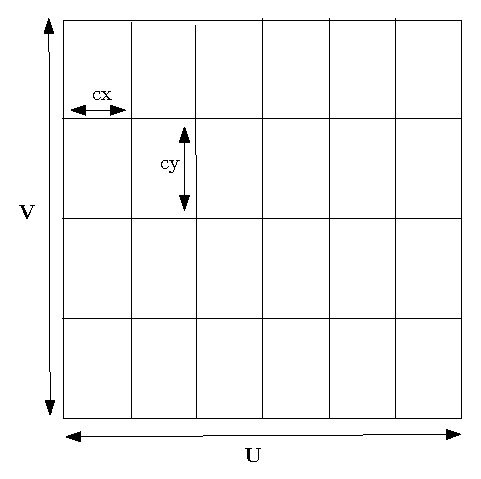
\includegraphics[width=90mm,scale=0.3]{hw_cells.eps}
\caption{Height and Width of Cells in the plane}
\end{center}
\end{figure} 
\subsection{Cancelable Template generation}
The protection of bit string is more important to secure the fingerprint template.The reason for this is,if the bit string is compromised, the vector $L_r$ will be revealed.So, it is important to convert bit string irreversibly.To solve this problem we transform the bit string $H_w$ into complex vector in the frequency domain by taking DFT.As the size of the bit string is B, we perform B-point discrete fourier transformation on $H_w$ to get its frequency domain complex vector.\\
\begin{equation}
D_i=\sum_{w=0}^{B -1} H_w e^{-j2\pi iw/B} , i=0,1,\ldots,B-1
\end{equation}
\\
We obtain a $D_i$ into the $B$x$1$ vector. $D=\{D_0,D_1,\ldots,D_{B-1}\}^{T}$. It is important to secure the complex vector ($D$).Next step is to transform $D$ into a non-invertible as in Wang and Hu(2012). Generate a user specific random matrix (R) using a user's PIN. $R$ is a $p$x$q$ matrix where $q=B$ and $p<q$ and T is the resulting vector of size $p$x$1$ transformed complex vector. The transformation is calculated as:\\
\begin{equation}
RD=T
\end{equation}
\paragraph{}
In a fingerprint image if the image contains $k$ number of minutiae then the fingerprint template contains $k$ 1D bit strings $T=\{ T_1,T_2,\ldots,T_k\}$. All these steps are repeated for the fingerprint that is to be verified, using the same user's PIN which generates the same random matrix in section 3.2. 

\subsection{Matching Score generation}
Fingerprint matching is matching the query fingerprint with the enrolled fingerprint and generate the matching score. This score ranges from 0 to 1. 0 being the total mismatch case and 1 being the perfect match case. This matching is a two step process: Global matching score and Local matching score generation.
\begin{figure}[htbp]
\begin{center}
\includegraphics[width=160mm,scale=0.75]{Matching_fig.eps}
\caption{Matching between query and enrolled Template($l\theta$ is the complex value of transformed L vector).}
\end{center}
\end{figure} 

\subsubsection{Local Matching score}
Let the enrolled fingerprint template be $T=\{T_1,T_2,\ldots,T_k\}$, where the fingerprint contains $k$-minutia and the query template be $T_q=\{T'_1,T'_2,\ldots,T'_m\}$, where $m$ is the number of minutia extracted from query template.\\
The distance between $T_i$ and $T'_j$ is described by:
\begin{equation}
d(T_i,T'_j)=\frac{\| T_i - T'_j\|_2}{\|T_i\|_2 +\|T'_j\|_2}
\end{equation}
where $\|.\|_2$ denotes the 2-norm of Gloub and Van Loan(1996). The matching score between the enrolled and queried template in the transformed domain is given by:\\
\begin{equation}
S(T_i,T'_j)=1-d(T_i,T'_j) 
\end{equation}
The value $S(T_i,T'_j)$ ranges from 0 to 1. Template generated of the same fingerprint with same reference minutiae will have a perfect match. But in the template we are not storing any information regarding the position of the reference minutiae. So we have compare every $T_i$ of $T=\{T_1,T_2\ldots,T_k\}$ with every $T'_j$ of $T'=\{T'_1,T'_2,\ldots,T'_m\}$. This will generate a similarity score matrix with dimensions $k$x$m$.  Each and every element of the similarity matrix is revisited and evaluated using the following conditions:
\begin{equation}
S(T_i,T'_j)=\left\{\def\arraystretch{1.2}%
  \begin{array}{@{}c@{\quad}l@{}}
    S(T_i,T'_j) & \text{Condition 1}\\
    0 & \text{Otherwise}\\
  \end{array}\right.
\end{equation}
where \textit{Condition 1} implies that $S(T_i,T'_j)$ must be maximum with respect to all the elements of the corresponding row and corresponding column.
\subsubsection{Global Matching Score}
The Global matching score of the enrolled and query template is given by :\\
\begin{equation}
MS=\frac{\sum_{i=1}^{k} \sum_{j=1}^{m}S(T_i,T'_j)}{\#S(T_i,T'_j)}
\end{equation}
where \# denotes the number of non-zero values jn the similarity matrix $S$. The matching score value ranges from 0 to 1, where 1 indicates a perfect match where as 0 indicates total mismatch between the enrolled and query template.
\section{Experimental results}
\subsection{Experimental setup}
The proposed method is tested using FVC 2002 DB1, DB2 and DB3 databases. Each of these databases contains 100 fingerprints and and each fingerprint has 8 impressions of which only 2 impressions are used to evaluate the proposed method. In total each database contains 800 images and we are using only 200 images in total. Neuro-Technology verifinger SDK \cite{13} is used to extract the fingerprint minutiae points from FVC 2002 DB1,DB2 and DB3.
\paragraph{}
The performance measures used for evaluation are False Acceptance Rate (FAR),False Rejection Rate(FRR) and Equal Error Rate(EER).  FRR is the probability of wrongly rejecting a genuine user as 
an imposter, where as FAR means wrongly accepting an imposter to be a genuine user. The value at which both FAR and FRR are equal is called the Equal Error Rate(EER). 
\paragraph{}
In our experimental setup, we used only two impressions of the 100 fingerprints in two databases, FVC 2002 DB1,FVC 2002 DB2. Genuine scores are calculated by matching one impression from the same fingerprint with the remaining impressions of the same fingerprint. This gives us a score set of 100 values for genuine scores. One impression of one fingerprint is matched with the all the impressions of remaining fingerprints to obtain imposter score distribution, which gives us a set of 19800 values for imposter scores. We will analyse the proposed method in terms of cancellable biometric template requirements:
\begin{itemize}
\item{Accuracy}
\item{Revocability}
\item{Irrevrsibilty}
\end{itemize}

\subsection{Revocability}
\paragraph{}
The fingerprint templates can be revoked by changing the user's PIN which intern changes the random matrix in the equation-$2$.  Diversity means when two different systems are using the same fingerprint template generation technique, the templates corresponding to the same fingerprint in the two systems should not correlate to each other, which means the template in one system when compared with a template in another system of the same fingerprint, should mark it as an imposter.
\paragraph{}
Diversity is tested by generating a pseudo imposter distribution. In this we have generated 200 templates with one key and another 200 templates with another key. The templates corresponding to the same fingerprint are matched to obtain the scores. It is noticed that the pseudo imposter distribution is close to imposter distribution. The mean and standard deviation of the imposter score distribution is $0.465$ and $0.06$ where as for imposter score generation these values are $0.579$ and $0.010$. From this result it can be observed that new transformed templates do not correlate to the compromised template even though they are impressions from the same fingerprint.
\subsection{Accuracy}
\paragraph{}
The performance measures used in this paper are FAR, FRR and EER. We have evaluated all these values for two databases FVC 2002 DB1 and FVC 2002 DB2. Figure 5: shows the Receiver Operating Characteristic(ROC) curve for DB1 and DB2. This curve is plotted against FAR and GAR, where GAR is  obtained by subtracting the values of FRR from 1, (GAR = 1-FRR). Figure 6: shows the EER calculation for the two databases. The point where the line  $y=x$  meets the curves is the EER point where FAR$ = $FRR (FMR=FNMR). The curve is plotted in logarithmic scale on both axes. In figure 7: shows the distribution of imposter and genuine scores for the database FVC 2002 DB1 using the same key for all users and the figure 8: shows the score distribution of FVC 2002 DB1 database when only the first $16$ distances are taken from the sorted distance vector. 
\paragraph{}
EER of the proposed method is $16.4\%$ for FVC 2002 DB1.   \\
The parameters used in the optimised result are:\\

\begin{tabular}{ l || r }

  \hline                       
  Length of bitstring& 2000 \\
  Maximum length & 400 \\
  Cx& 7 \\
  Cy & 10\\
  \hline  
\end{tabular}

\begin{figure}[htbp]
\begin{center}
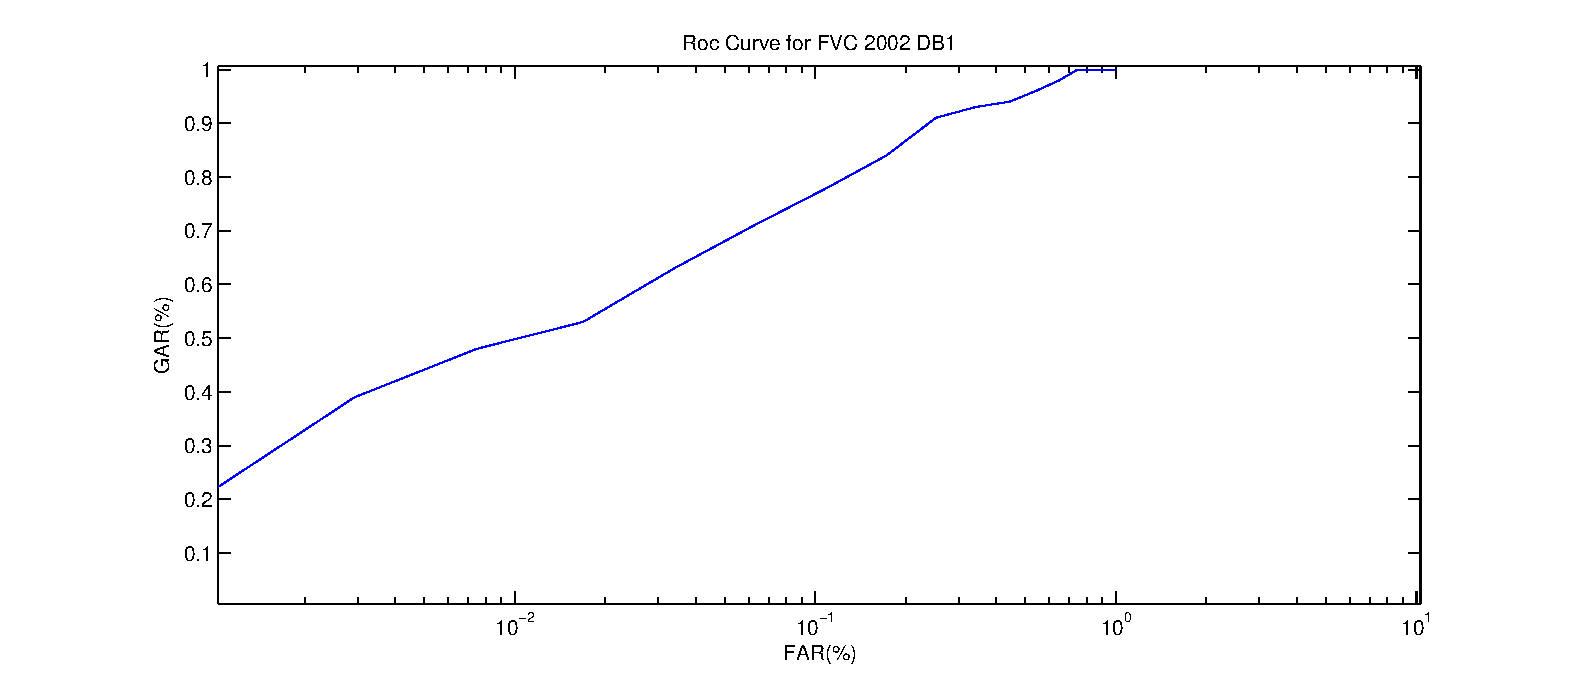
\includegraphics[width=180mm,scale=0.5]{FVC2002_DB1_ROC.eps}
\caption{ROC Curve.}
\end{center}
\end{figure} 

\begin{figure}[htbp]
\begin{center}
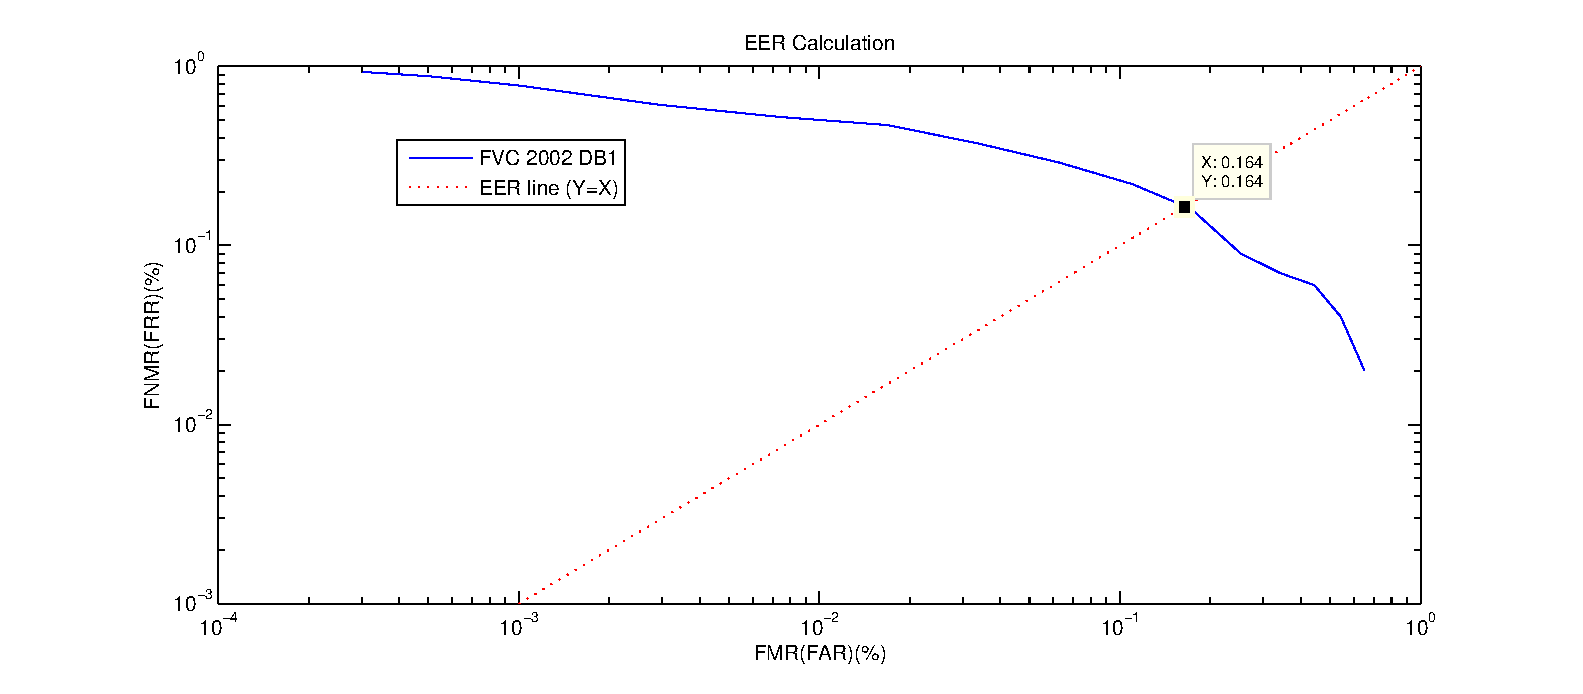
\includegraphics[width=180mm,scale=0.5]{EERf.eps}
\caption{EER Calculation of FVC 2002 DB1 database .}
\end{center}
\end{figure} 

\begin{figure}[htbp]
\begin{center}
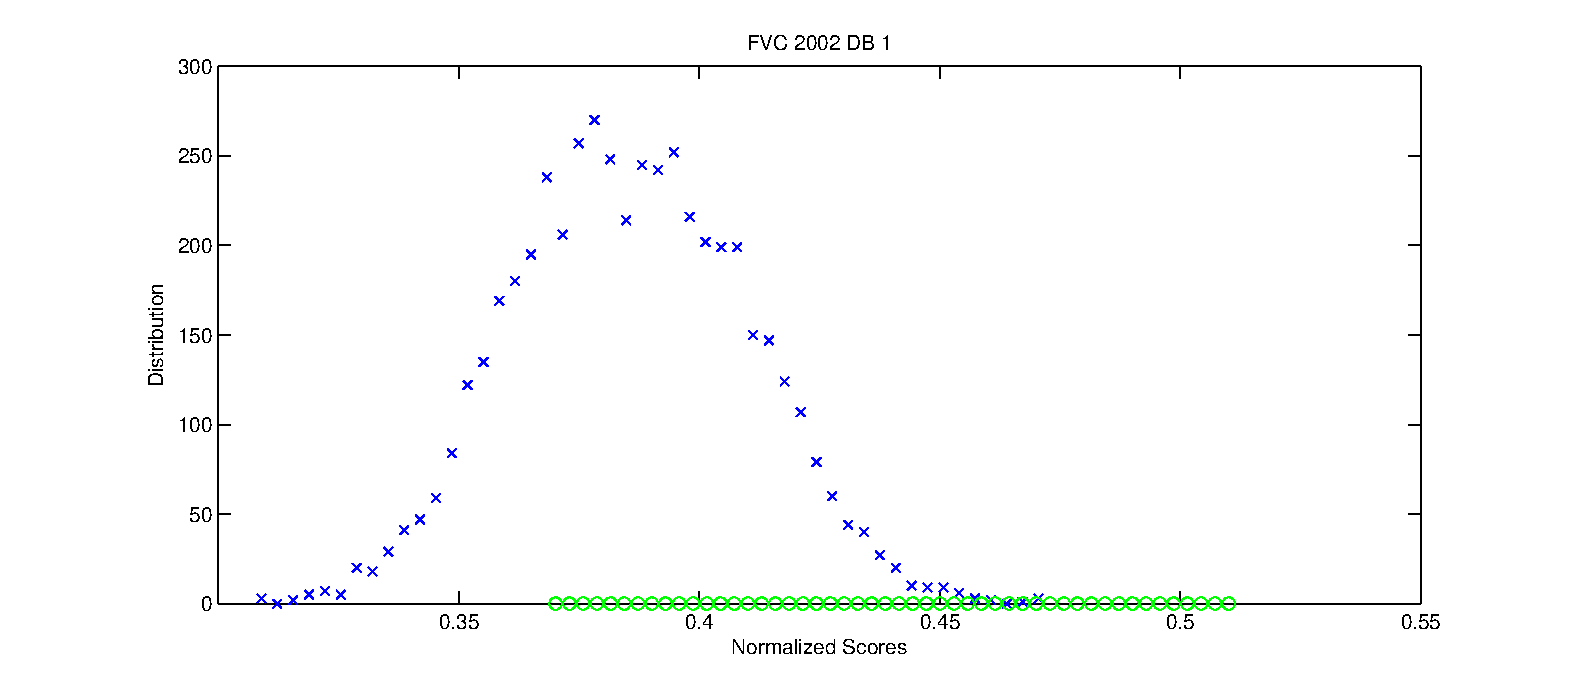
\includegraphics[width=180mm,scale=0.5]{Scoredisf.eps}
\caption{Score Distribution of FVC 2002 DB1 using same key for all users(all).}
\end{center}
\end{figure} 

\begin{figure}[htbp]
\begin{center}
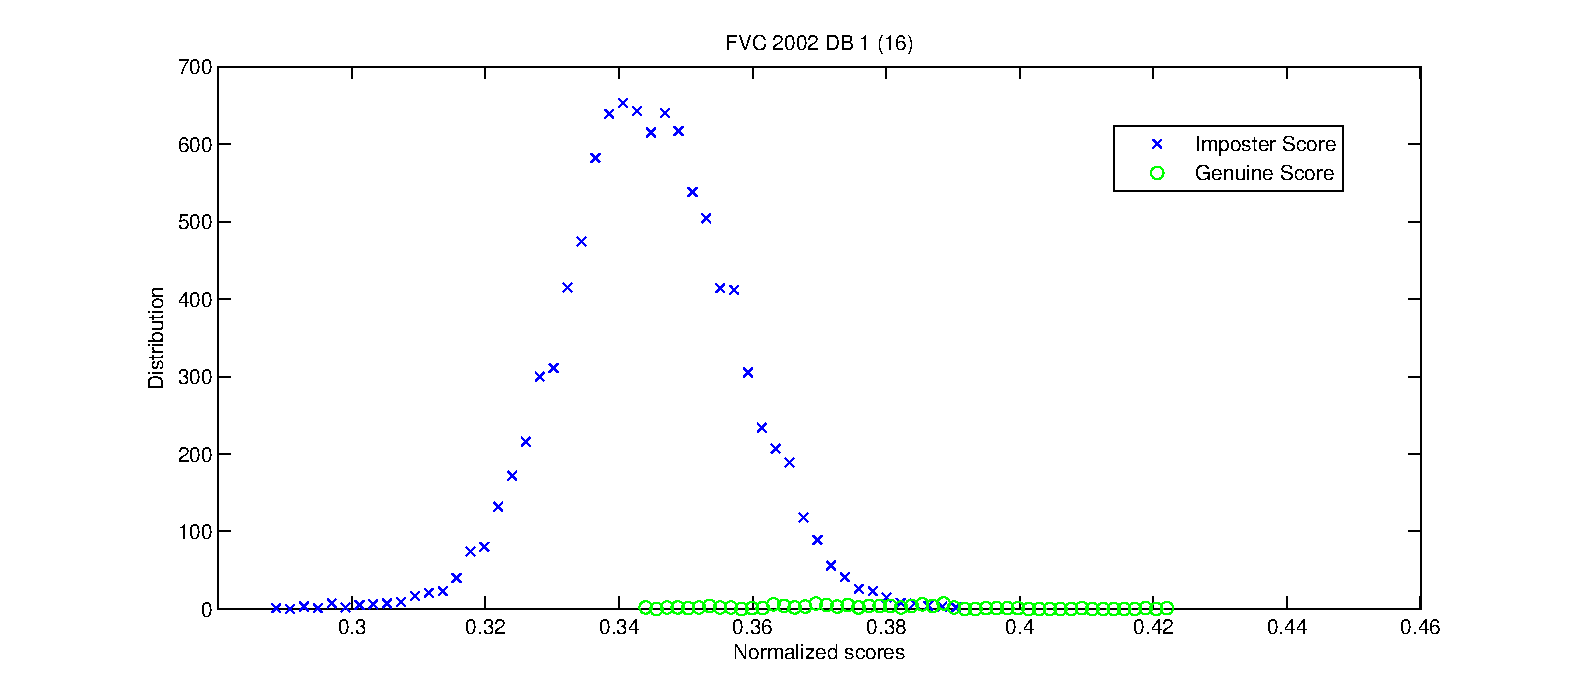
\includegraphics[width=180mm,scale=0.5]{Scoredisf2.eps}
\caption{Score Distribution of FVC 2002 DB1 using same key for all users(n=16).}
\end{center}
\end{figure} 



\subsection{Irreversibility}
Irreversibility is the primary requirement of cancelable biometrics, which means it is computationally impossible to reverse a given template. If the bit string ($H_w$) is compromised, it is not possible to reconstruct $L_r$ from the $H_w$ because of the quantisation applied on the $L_r$ before converting it to bit string $H_w$. 
\paragraph{}
Case A: If the attacker is able to obtain the $L_r$ vector, then we will show how it is computationally impossible to obtain the original fingerprint features. In the $L_r$ vector, we are storing the leg distances of the contiguous right angle triangles formed by the distances of the minutiae from the reference minutiae. As the attacker knows only the value of one side in a right angled triangle, he have to make a guess regarding the other two sides. In the worst case, if the attacker is able to figure out correctly the other two sides, then he knows the distance of all minutia from reference minutiae. But we are not storing the location of reference minutiae, so he has to choose a position for the reference minutiae. Also we are storing the relative minutiae orientation, he has to again guess the orientation of the reference minutiae. The average distance between neighbouring minutiae is $65$ pixels. The size of the images in FVC 2002 database are of the range $256$x$520$. So the total number of attempts required are 296 x 520 x $2\pi$ x 65 $\approx$ 67 million. Each spiral contains all the minutia of the fingerprint, and each fingerprint contains atleast 10 minutia. So the total number of attempts required are $10$ x $67$ million $\approx 6.7$ billion.
\paragraph{}
Case B: Assume that the attacker knows the bit string and the quantisation cell size on the plane. In worst case scenario if every cell of the plane contains a point and the plane size is $U$X$V$(38 x 36) for FVC 2002 DB1 and 70 x 36 for FVC 2002 DB2. So the total number of attempts if the image size is 296 x 560, is 296 x 560 x 38 x 36 $\approx$ 225 million for FVC 2002 DB1 and for FVC 2002 DB2 it is 296 x 560 x 70 x 36 $\approx$ 430 million are required to guess the minutia location from the bit string($H_w$).

\section{Conclusion}
In this paper we proposed a alignment free template generation technique. We have used the invariant features from the construction of spiral and relative orientations. These features are used to generate bit string based on plane based quantization. The performance of the method is evaluated using FVC 2002 DB1. The EER for the DB1 is $16.4\%$.
\begin{thebibliography}{9}

\bibitem{1}
  \emph{ Introduction to Biometrics}, Anil K. Jain,Arun A.Ross,Karthik Nandakumar, Springer, 2011.
\bibitem{2}
\emph{A survey on biometric cryptosystems and cancelable biometrics}, Rathgeb, Christian and Uhl, Andreas,   Volume 2011,Number 1, edition 3, \emph{EURASIP Journal on Information Security}, 2011,10.1186/1687-417X-2011-3, Springer International Publishing AG.
\bibitem{3}
\emph{Fingerprint image reconstruction from standard Templates}, Cappelli R., Maio D., Lumini A., Maltoni D., 2007, IEEE Transactions on Pattern Analysis and Machine Intelligence 29, 1489-503
\bibitem{4}
\emph{ Fingerprint Shell: Secure Representation of Fingerprint Template}, Moujahdi C., Bebis G., Ghouzali S., Rziza M., Pattern Recognition Letters(2014),\emph{doi: http://dx.doi.org/10.1016/j.patrec.2014.04.001}
\bibitem{5}
N.K. Ratha, S. Chikkerur, J.H. Connell, R.M. Bolle, \emph{Generating cancelable fingerprint templates}, IEEE Transactions on Pattern Analysis and Machine Intelligence 29 (4) (2007) 561?572.
\bibitem{6}
Q. Feng, F. Su, A. Cai, \emph{Cracking Cancelable Fingerprint Template of Ratha, in: The International Symposium on Computer Science and Computational Technology (ISCSCT?08)}, 2008, pp. 572?575.
\bibitem{7}
S.W. Shin, M.-K. Lee, D. Moon, K. Moon, \emph{Dictionary attack on functional transform-based cancelable fingerprint templates}, ETRI Journal 31 (5) (2009) 628-630.
\bibitem{8}
Song Wang, Jiankun Hu, \emph{Alignment-free cancelable fingerprint template design: A densely infinite-to-one mapping(DITOM) approach}, Pattern Recognition 45(2012) 4129-4137
\bibitem{9}
R. Cappelli, M. Ferrara, D. Maltoni, \emph{Minutia Cylinder Code : a new representation and matching technique for fingerprint recognition}, IEEE Transactions on Pattern Analysis and Machine Intelligence, 32(12) (2010) 2128-2141
\bibitem{10}
M. Ferrara, R. Cappelli, D. Maltoni,\emph{ Non-invertible minutia cylinder code representation}, IEEE Transactions on Inf. Forensics security 7(6) (2012) 1727-1737
\bibitem{11}
C. Lee, J. Kim, \emph{Cancelable fingerprint templates using minutia-based bit-strings}, Journal of Network and Computer Applications, 33 (3) (2010) 236-246
\bibitem{12} 
Prasad, M.V.N.K, Santhosh kumar C., Fingerprint Template protection using multiline neighbouring relation, Expert Systems with Applications(2014), http://dx.doi.org/10.1016/j.eswa.2014.04.020
\bibitem{13}
Neurotechnology Veri-Finger SDK, Trail version - 6.7.



\end{thebibliography}





\end{document}